% Research Paper for GECCO 2015
% by Nic McPhee, Kirbie Dramdahl, and David Donatucci

\documentclass{sig-alternate}

\usepackage{parskip}
\usepackage{times} %For typeface
\usepackage{graphicx}
\usepackage{algorithm}
\usepackage{algorithm,algorithmic}
\usepackage[justification=centering]{caption}[2007/12/23]
\usepackage{url}
\sloppy

\setlength{\parindent}{0.5cm} 

\newcommand{\citep}[1]{\cite{#1}}

\DeclareGraphicsRule{.tif}{png}{.png}{`convert #1 `dirname #1`/`basename #1 .tif`.png}

\begin{document}

\conferenceinfo{GECCO'15,} {July 11-15, 2015, Madrid, Spain.}
\CopyrightYear{2015}
\crdata{TBA}
\clubpenalty=10000
\widowpenalty = 10000
    
\title{Impact of Crossover Bias in Genetic Programming}

\numberofauthors{1}
\author{
\alignauthor
Nicholas Freitag McPhee, M. Kirbie Dramdahl, David Donatucci\\
	\affaddr{Division of Science and Mathematics}\\
	\affaddr{University of Minnesota, Morris}\\
	\affaddr{Morris, MN USA-56267}\\
	\email{\{mcphee, dramd002, donat056\}@morris.umn.edu}
}

% This is more like how it "should" be done, but I think the previous approach might look nicer. They
% may force us to change it, though, to make it easier to scrape information.

%\numberofauthors{3}
%\author{
%\alignauthor
%Nicholas Freitag McPhee\\
%	\affaddr{Division of Science and Mathematics}\\
%	\affaddr{University of Minnesota, Morris}\\
%	\affaddr{Morris, MN USA-56267}\\
%	\email{mcphee@morris.umn.edu}
%\alignauthor
%M. Kirbie Dramdahl\\
%	\affaddr{Division of Science and Mathematics}\\
%	\affaddr{University of Minnesota, Morris}\\
%	\affaddr{Morris, MN USA-56267}\\
%	\email{dramd002@morris.umn.edu}
%\alignauthor
%David Donatucci\\
%	\affaddr{Division of Science and Mathematics}\\
%	\affaddr{University of Minnesota, Morris}\\
%	\affaddr{Morris, MN USA-56267}\\
%	\email{donat056@morris.umn.edu}
%}

\date{} 
    
\maketitle

\begin{abstract}

\emph{\scriptsize This is probably too long. People often recommend keeping the abstract to somewhere 
between 150 and 250 words, and this is closer to 500. For the initial submission that's OK, but we may want 
to move some of this to the introduction and trim down the abstract somewhat.}

In tree-based genetic programming with sub-tree crossover, the parent contributing the root portion of the tree 
(which 
we refer to as the \emph{root parent}) often contributes more to the semantics of the resulting child than the 
other parent (the 
\emph{non-root parent}). In previous research, we found that when the root parent had greater fitness 
than the 
non-root parent, the fitness of the child tended to be better than if the reverse were true. Here we explore the 
significance of that asymmetry by introducing the notion of \emph{crossover bias}, which allows us to bias the 
system 
in favor of having the more fit parent be the root parent. To better understand the impact of this bias, 
we implemented several levels 
of 
crossover bias, including 0\% bias 
(root individual chosen randomly, as in traditional sub-tree crossover), 
100\% bias (the stronger parent is always chosen to be the root parent), 
50\% bias 
(bias implemented in half 
the cases, and the other half chosen randomly), and reverse bias (the weaker parent is always chosen 
as root parent). 

We applied crossover bias to a variety of problems. In most cases we found that using crossover bias 
either improved performance or had no impact. 
Our results do, however, indicate the possibility that 
crossover bias may increase selection pressure and premature convergence -- undesirable behavior, as it 
encourages a genetic programming run to arrive at a solution too quickly, in the process potentially excluding 
more accurate solutions for a more generalized one.

Our results also demonstrate that the effectiveness of 
crossover bias is somewhat dependent on the problem, and significantly dependent on other parameter 
choices. In 
particular it appears that crossover bias has the largest impact when selection pressure is weaker, and the 
differences 
in the fitness of the parents is thus likely to be larger. We also found that the use of elitism 
reduced the influence of crossover bias. It's possible that crossover bias acts to some degree as an 
``elitism'' operator, making it more likely that the semantics of more fit individuals are copied into the next 
generation; 
thus if traditional elitism is being employed this effect is less visible. Another possible explanation for this is 
that if the most fit individuals are automatically being carried over, there is perhaps less need to produce new, 
fitter individuals via crossover, reducing or even eliminating the usefulness of crossover bias. Other factors 
which we found to have potential impact on the effectiveness of crossover bias were tournament size, 
population size, and possibly the difference in parental fitness.

\end{abstract}

\category{}{}{}
\terms{}
\keywords{genetic programming, crossover bias, root parent}

\section{Introduction} \label{sec:Introduction}

\textbf{Nic should try to capture some nice things Lee Spector said about the importance of asymmetrical 
recombination operators (which are very common in biology, e.g., sex-linked traits) and how we've identified an 
asymmetry in subtree crossover and a way to potentially exploit that.}

\section{Crossover Bias} \label{sec:XObias}

In tree-based genetic programming, sub-tree crossover remains a very common reproduction mechanism 
\cite{poli08:fieldguide}. As Figure~\ref{fig:root_parent_illustration} illustrates, sub-tree crossover is an inherently 
asymmetric operation, with one parent contributing the root node and, in most cases, a substantially larger total 
number of nodes than the other parent. In this work we will refer to the individual which contributes the root node as 
the \emph{root parent} and the other as the \emph{non-root parent}. 

\begin{figure}
\centering
\includegraphics[width=0.45 \textwidth]{Plots/Root_parent_illustration.pdf}
\caption{Sub-tree crossover, illustrating the asymmetric role of the \emph{root} and \emph{non-root} parents.}
\label{fig:root_parent_illustration}
\end{figure}

Crucial to this work, it has been previously noted \cite{McPheeDonatucciDramdahl:2014, McPhee:2008:SBB:
1792694.1792707} that in many cases the root parent also tends to contribute more to the semantics of the resulting 
individual than the non-root parent. This is in part because of the tendency of the root parent to contribute more 
overall nodes, but is also because for most function sets the root node (and the nodes near it) have an especially 
strong impact on the result of evaluating the tree in question. While the details and impact of this asymmetry will 
depend a great deal on the details of the function set and the particular trees chosen as parents, in many common 
tree-based GP settings the asymmetry has a quite substantial impact on the semantics of the offspring.

While this paper focuses on the asymmetry in the context of tree-based GP and sub-tree crossover, it's important to 
note that asymmetries like this are common in many evolutionary systems, both biological and artificial. Much 
eukaryote reproduction is sexual, and brings with it numerous sex-linked traits and related asymmetries, for example. 
\textbf{Do we want a bib entry here? Something as simple as a Wikipedia reference, or something ``fancier'' like a 
review article on sex-linked traits?} Many evolutionary computation systems other than tree-based GP also have 
significant asymmetries. Many linear GP systems (\textbf{cite something - Wolfgang's book?}) and stack-based GP 
systems (\textbf{cite PUSH}), for example, have asymmetries where the last instructions executed can have a 
disproportionate impact on the results, and changes near the front of a grammatical evolution strings will have a 
disproportionate impact by determining the important early choices in the grammar productions. In general these 
asymmetries weren't intentional design goals, but were instead simple artifacts of other system design decisions, and 
the potential impact of these asymmetries has been largely unstudied.

In previous work~\cite{McPheeDonatucciDramdahl:2014} recording individual ancestry in tree-based genetic 
programming,
it was found that if the root parent had a greater fitness (a better-fitting solution to the problem being solved) than
the non-root parent, the fitness of the individual produced tended to be greater than in the reverse scenario. In this
work, in order to further research this occurrence, we implemented what we refer to crossover bias, which allowed us 
to
force the genetic programming system to assign the individual with the greater fitness to be the root parent in a
certain percentage of cases.

\textbf{I'm starting to think that most of the preceding text in this section really belongs in the introduction, leaving this section to focus on the details of how we implemented XO bias. Thoughts?}
For this work, we implemented six levels of crossover bias:
\begin{itemize}
\item -1 bias - system forced to always select the less fit parent as the root parent, also referred to as reverse bias;
\item 0 bias - no crossover bias occurred, also referred to as no bias;
\item 0.25 bias - system forced to select the more fit parent as the root parent in 25\% of cases;
\item 0.50 bias - system forced to select the more fit parent as the root parent in 50\% of cases;
\item 0.75 bias - system forced to select the more fit parent as the root parent in 75\% of cases; and
\item 1 bias - system forced to always select the more fit parent as the root parent, as referred to as simply bias.
\end{itemize}

\section{Experimental Setup} \label{sec:Experiments}

\textbf{Talk about the fact that we used pairwise Wilcoxon test with Holm corrections for the bulk of our statistical 
tests, along with a reference/citation to R as generated inside R. I'm not sure if we want to mention pairwise test of 
proportions (chi-squared) or not, because I'm not sure how much we'll use it in the paper.}

In the following sections, the terms ``bias-effective settings'' and ``non-bias-effective settings'' are used to
describe specific settings used in collecting data from runs. These terms are defined here, for convenience.

Bias-effective settings were as follows:
\begin{itemize}
\item binary tournaments,
\item no elitism, and
\item population size of 10,240;
\end{itemize}
and are so named because, with these settings in place, crossover bias tended to have the strongest effect.

Non-bias-effective settings, conversely, were as follows:
\begin{itemize}
\item tournament sizes of seven individuals,
\item elitism of either 0.1\% or 1\%, and
\item population size of 1,024;
\end{itemize}
and are so named because, with these settings in place, crossover bias tended to have the weakest effect.

\section{Results} \label{sec:Results}

\subsection{Structural Problems}

\subsubsection{K-Landscapes Problems}

We did a full sweep of parameters for the K-Landscapes problem with both $K=2$ and $K=6$, using various combinations of the following:

\begin{itemize}
	\item crossover biases of -1, 0, 0.25, 0.5, 0.75, and 1;
	\item population sizes of 1,024 and 10,240;
	\item elitism percentages of 0\% or 1\%; and
	\item tournament sizes of 2, 3, 5, and 7.
\end{itemize}

Figure~\ref{fig:KLandscapes6_results} shows the impact of crossover bias on this problem across all the 
combinations of parameter values (excepting reverse bias). Increasing the amount of crossover bias consistently
improves the fitness of the results. All the differences are statistically significant ($p < 0.012$) except for the
difference between bias probability 0.75 and 1.0.

%> pairwise.wilcox.test(klandscapes6$Fitness, klandscapes6$Bias.probability)
%
%	Pairwise comparisons using Wilcoxon rank sum test 
%
%data:  klandscapes6$Fitness and klandscapes6$Bias.probability 
%
%     -1      0       0.25    0.5     0.75   
%0    0.99997 -       -       -       -      
%0.25 1.8e-06 1.8e-06 -       -       -      
%0.5  1.7e-12 2.3e-12 0.01136 -       -      
%0.75 < 2e-16 < 2e-16 6.0e-10 0.00032 -      
%1    < 2e-16 < 2e-16 3.7e-15 2.2e-07 0.15773
%
%P value adjustment method: holm 

\begin{figure}
\centering
\includegraphics[width=0.45 \textwidth]{Plots/KLandscapes6_XO_bias_impact_transformed_boxplot_alpha075.pdf}
\caption{Impact of crossover bias on fitness for K-Landscapes problem, $K=6$ for a variety of treatments.}
\label{fig:KLandscapes6_results}
\end{figure}

Figure~\ref{fig:KLandscapes6_strong_results} filters out only the data gathered using the bias-effective treatment,
discussed in Section~\ref{sec:Experiments}. It is clear that the impact of crossover bias is much stronger in this case
than in the more general case shown in Figure~\ref{fig:KLandscapes6_results}. Here all the differences are strongly
statistically significant ($p < 10^{-11}$), with the exception of the difference between reverse bias (-1; not shown)
and no bias (0). In addition to improvements in fitness, increasing the crossover bias also increases the number of
``perfect'' solutions discovered. Out of 100 runs with a crossover bias setting of 1, 15 of these runs resulted in the
discovery of a ``perfect'' solution. By comparison, only 1 or 2 runs out of 100 resulted in ``perfect'' solutions for
each of the other crossover probabilities. This difference is statistically significant with $p \leq 0.03$ using a
pairwise test of proportions.

\begin{figure}
\centering
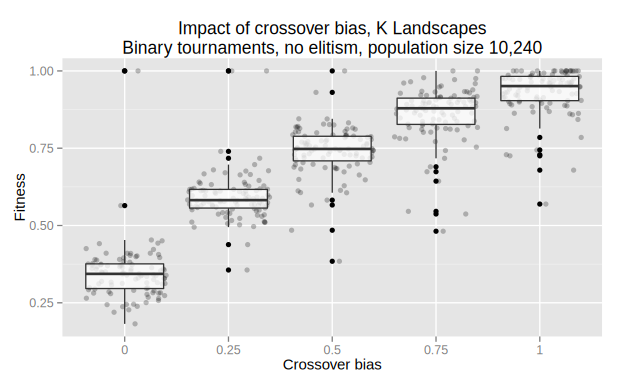
\includegraphics[width=0.45 \textwidth]{Plots/KLandscapes6_XO_bias_strong_impact_alpha_075.pdf}
\caption{Impact of crossover bias on fitness for K-Landscapes problem, $K=6$, restricted to binary tournament 
selection, no elitism, and population size 10,240.}
\label{fig:KLandscapes6_strong_results}
\end{figure}

%> pairwise.wilcox.test(strong$Fitness, strong$Bias.probability)
%
%	Pairwise comparisons using Wilcoxon rank sum test 
%
%data:  strong$Fitness and strong$Bias.probability 
%
%     -1      0       0.25    0.5     0.75   
%0    0.18    -       -       -       -      
%0.25 < 2e-16 < 2e-16 -       -       -      
%0.5  < 2e-16 < 2e-16 < 2e-16 -       -      
%0.75 < 2e-16 < 2e-16 < 2e-16 < 2e-16 -      
%1    < 2e-16 < 2e-16 < 2e-16 < 2e-16 2.3e-12
%
%P value adjustment method: holm 

%> countSuccesses(strong)
%[1]  1  2  2  1  2 15
%> pairwise.prop.test(countSuccesses(strong), rep(100, 6))
%
%	Pairwise comparisons using Pairwise comparison of proportions 
%
%data:  countSuccesses(strong) out of rep(100, 6) 
%
%  1     2     3     4     5    
%2 1.000 -     -     -     -    
%3 1.000 1.000 -     -     -    
%4 1.000 1.000 1.000 -     -    
%5 1.000 1.000 1.000 1.000 -    
%6 0.011 0.030 0.030 0.011 0.030
%
%P value adjustment method: holm 

\subsubsection{Ordertree Problem}

\textbf{Everything in this section at the moment is really just Nic chatting about the results that we have, hoping for 
some ideas/feedback from Kirbie and David. Thoughts, suggestions, questions, changes, actual usable text, etc., all 
greatly appreciated.}

For the OrderTree problem, a full sweep of the following parameters was used:

\begin{itemize}
	\item crossover biases of -1, 0, 0.25, 0.5, 0.75, and 1;
	\item population size of 1,024;
	\item elitism percentages of 0\% or 1\%; and
	\item tournament sizes of 2, 3, 5, and 7.
\end{itemize}

While similar to the parameters used for the K-Landscapes problem, one difference is apparent: the population size for
the OrderTree runs was limited to 1,024. This was a consequence of the large trees generated for this problem,
resulting in out of memory errors for the larger population size of 10,240.

Initial runs of this problem with (1) and without (0) crossover bias across all four tournament sizes demonstrated that
in each case, adding crossover bias improved fitness. Additionally, these improvements were statistically significant
($p < 0.002$ for each pairing using a pairwise Wilcoxon with Holm correction).

However, in the next set of runs, using the full range of crossover bias values but limited to binary tournaments, we
observed a drop in fitness from bias 0.75 to bias 1, actually dropping slightly below that for 0.50 as well. All these
differences are statistically significant ($p < 0.03$), with the exception of the difference between bias 0.25 and bias
1, so bias 0.75 is the clear winner in this scenario. \textbf{I (Nic) suspect this is actually quite interesting and
might open interesting doors to things like premature convergence and need for being able to have a least a little
variation in the system for a problem like this. Maybe we should talk about that in the "Future work" section?}

Figure~\ref{fig:Ordertree_results_all_tournaments_Jan15} generalizes this to cover all four tournament sizes. The
figure demonstrates that the drop in fitness for bias 1 observed for binary tournaments is consistent across the other
three tournament sizes as well. However, it is also apparent from the figure that in general the impact of crossover
bias lessens with the larger tournament sizes, both in the increase in fitness up to bias 0.75, and the drop from there
to bias 1.

\begin{figure}
\centering
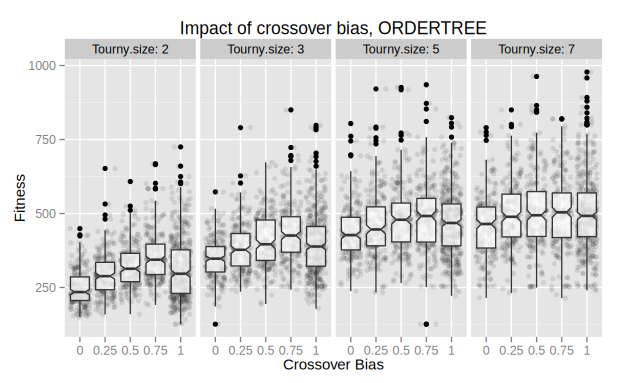
\includegraphics[width=0.45 \textwidth]{Plots/Ordertree_results_all_tournaments_Jan15.pdf}
\caption{Impact of crossover bias on fitness for Ordertree problem for multiple tournament sizes.}
\label{fig:Ordertree_results_all_tournaments_Jan15}
\end{figure}

Compare this to the results shown in Figure~\ref{fig:KLandscapes6_XO_bias_impact_facets}, which plots the corresponding
data from the K-Landscapes runs. It is clear that for binary tournaments, increasing the crossover bias probability
continues to improve the fitness - all the differences are strongly statistically significant ($p<6e-08$). This
continues to be true for tournament size 3 - all the differences are statistically significant except for that between
bias 0.50 and 0.75 and that was very close ($p=0.05620$). None of the differences for tournament size 5 are
significant, and so we will past over it here. For tournament 7, however, it does look like the reverse is true, where
increasing crossover actually hurts fitness. Almost none of the differences for tournament size 7 are statistically
significant, however, with the only exception being the difference between 0.25 and 1 ($p=0.21$ using a pairwise
Wilcoxon test with Holm correction). \textbf{This paragraph might move to the Discussion or Conclusions section if we
keep it, or something like it.}

\begin{figure}
\centering
\includegraphics[width=0.45 \textwidth]{Plots/KLandscapes6_XO_bias_impact_facets.pdf}
\caption{Impact of crossover bias on fitness for K-Landcapes problem, K=6, for various tournament sizes.}
\label{fig:KLandscapes6_XO_bias_impact_facets}
\end{figure}

%> pairwise.wilcox.test(subset(klandscapes6, Tourny.size==7)$Fitness, subset(klandscapes6, Tourny.size==7)$Bias.probability)
%
%	Pairwise comparisons using Wilcoxon rank sum test 
%
%data:  subset(klandscapes6, Tourny.size == 7)$Fitness and subset(klandscapes6, Tourny.size == 7)$Bias.probability 
%
%     0     0.25  0.5   0.75 
%0.25 1.000 -     -     -    
%0.5  1.000 1.000 -     -    
%0.75 1.000 0.556 1.000 -    
%1    0.075 0.021 0.556 1.000
%
%P value adjustment method: holm 

\subsection{U.S. Change Problem}

For the U.S. Change problem, we'll use ``Hits'' (the number of test cases that are correctly solved) as the measure of 
the success of a run. There are 150 test cases in our implementation, so an optimal program will have a ``Hits'' score 
of 150.

Figure~\ref{fig:USChange_Hits} shows the impact of crossover bias on the number of hits for the U.S. Change 
problem across the full collection of parameter settings. This suggests that in in general there is little consistent 
impact of crossover bias, but a pairwise Wilcoxon test with Holm correction indicates that while most of the 
differences in this plot aren't statistically significant, two are: The differences between crossover bias 0 and crossover 
bias 0.5 and 0.75 are both statistically significant ($p \leq 0.015$), even if numerically small.

\begin{figure}
\centering
\includegraphics[width=0.45 \textwidth]{Plots/US_change_hits.pdf}
\caption{Impact of crossover bias on the number of hits for the US Change problem.}
\label{fig:USChange_Hits}
\end{figure}

%> pairwise.wilcox.test(us_change$Hits, us_change$Bias, conf.int=TRUE)
%
%	Pairwise comparisons using Wilcoxon rank sum test 
%
%data:  us_change$Hits and us_change$Bias 
%
%     0     0.25  0.5   0.75 
%0.25 0.117 -     -     -    
%0.5  0.011 1.000 -     -    
%0.75 0.015 1.000 1.000 -    
%1    0.083 1.000 1.000 1.000
%
%P value adjustment method: holm 

If we limit our attention to binary tournaments, no elitism, and the larger population size (10,240), then we find that 
crossover bias has a substantial and statistically significant impact, as is seen in Figure~
\ref{fig:USChange_Hits_strong}. Here the bulk of these pairwise differences are statistically significant ($p<0.0002$ 
using a pairwise Wilcoxon test with Holm correction). The major exception is the difference between crossover bias 
0.75 and 1.0 ($p=0.43078$). Two other adjacent pairs have $p$-values slightly above 0.05: Crossover bias 0.25 
\emph{vs.} 0.5 ($p=0.05036$), and 0.5 \emph{vs.} 0.75 ($p=0.08019$). \textbf{We could put all the $p$ values in a 
table, bolding the ones that are significant. This is somewhat common in the literature, but would use quite a bit more 
space, especially since half the table would be empty. Thoughts?}

\begin{figure}
\centering
\includegraphics[width=0.45 \textwidth]{Plots/US_change_hits_strong.pdf}
\caption{Impact of crossover bias on the number of hits for the US Change problem, limited to binary 
tournaments, no elitism, and population size 10,240.}
\label{fig:USChange_Hits_strong}
\end{figure}

%> pairwise.wilcox.test(us_change_strong$Hits, us_change_strong$Bias)
%
%	Pairwise comparisons using Wilcoxon rank sum test 
%
%data:  us_change_strong$Hits and us_change_strong$Bias 
%
%     0       0.25    0.5     0.75   
%0.25 0.00013 -       -       -      
%0.5  3.4e-09 0.05036 -       -      
%0.75 1.1e-12 0.00016 0.08019 -      
%1    3.2e-15 5.1e-06 0.01652 0.43078
%
%P value adjustment method: holm 

If complete success was considered vital (which might be the case if we were evolving software for use in a 
production system), then it would make sense to see if crossover bias has a significant impact on the success rate. 
Figure~\ref{fig:USChange_Successes_strong} shows the number of successes for the various crossover bias values 
when using binary tournaments, no elitism, and population size 10.240. A pairwise test of proportions (chi-squared) 
with Holm correction indicates that while non of the adjacent differences (e.g., crossover bias 0.5 \emph{vs.} 0.75) are 
statistically significant, most of the non-adjacent differences (e.g., crossover bias 0.25 \emph{vs.} 0.75) are 
statistically significant, with the exceptions being crossover bias 0 \emph{vs.} 0.5, and bias 0.5 and 1.0 ($p=0.09361$ 
in both cases). 

\begin{figure}
\centering
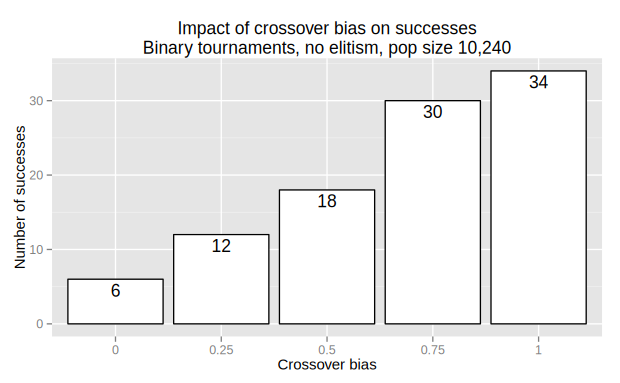
\includegraphics[width=0.45 \textwidth]{Plots/US_change_successes_strong.pdf}
\caption{Impact of crossover bias on the number of successes runs for the US Change problem when using 
binary tournaments, no elitism, and population size 10,240.}
\label{fig:USChange_Successes_strong}
\end{figure}

%> pairwise.prop.test(c(6, 12, 18, 30, 34), rep(100, 5))
%
%	Pairwise comparisons using Pairwise comparison of proportions 
%
%data:  c(6, 12, 18, 30, 34) out of rep(100, 5) 
%
%  1       2       3       4      
%2 0.65003 -       -       -      
%3 0.09361 0.65003 -       -      
%4 0.00021 0.02215 0.27429 -      
%5 1.8e-05 0.00334 0.09361 0.65003
%
%P value adjustment method: holm 

%\begin{figure}
%\centering
%\includegraphics[width=0.45 \textwidth]{Plots/US_change_Bias_impact_vs_success.png}
%\caption{Relationship between proportion of successful runs and the impact of crossover bias.}
%\label{fig:USChangeBiasImpactVsSuccess}
%\end{figure}

\subsection{Symbolic Regression Problems}

\subsubsection{Pagie-1 Problem}

\textbf{How do we want to handle the quite substantial difference in the behavior of the two different function sets? It 
could be argued that it's not really our fight and that we can/should just pick one and go with it and not get all bogged 
down in trying to explain the differences between these and why they behave so differently. But if we just pick one, it 
kind of smells like cherry picking. The basic4 set clearly has the stronger ``bias is bad'' result for tournament size 7. If 
we keep both of function sets we also open the door to a discussion of the value of focusing on hits vs. error, which is 
another discussion I'm to sure we want to get distracted by here. Thoughts?}

Figure~\ref{fig:Pagie1Hits_Bias_Tournys_FunctionSet} shows the impact of crossover bias on the number of hits for 
the Pagie-1 regression problem, separated out by both tournament size and function set used; Figure~
\ref{fig:Pagie1Fitness_Bias_Tournys_FunctionSet} is similar, but plots fitness (total error) instead of hits.

\begin{figure}
\centering
\includegraphics[width=0.45 \textwidth]{Plots/Pagie_1_Hits_vs_Bias_Tournys_FunctionSet.pdf}
\caption{Impact of crossover bias on the number of hits for the Pagie-1 symbolic regression problem, broken out for 
the four different tournament sizes (2, 3, 5, and 7) and the two different function sets (basic4 and koza2). The 
maximum number of possible hits is 676.}
\label{fig:Pagie1Hits_Bias_Tournys_FunctionSet}
\end{figure}

\begin{figure}
\centering
\includegraphics[width=0.45 \textwidth]{Plots/Pagie_1_Fitness_vs_Bias_Tournys_FunctionSet.pdf}
\caption{Impact of crossover bias on the fitness (total error) for the Pagie-1 symbolic regression problem, broken out 
for the four different tournament sizes (2, 3, 5, and 7) and the two different function sets (basic4 and koza2). The best 
possible is an error of 0.}
\label{fig:Pagie1Fitness_Bias_Tournys_FunctionSet}
\end{figure}

\textbf{The following parameter settings that seem to generate the clearest impact of crossover bias:}
\begin{itemize}
	\item ``basic4'' function set (just $+, -, \times, \div$)
	\item No elitism
	\item Large population (10,240)
	\item Tarpeian bloat control
\end{itemize}
\textbf{If we limit ourselves to these settings, then the complexities of Figures~
\ref{fig:Pagie1Hits_Bias_Tournys_FunctionSet} and~\ref{fig:Pagie1Fitness_Bias_Tournys_FunctionSet} simplify to 
Figures~\ref{fig:Pagie1StrongHits_Bias_Tournys_FunctionSet} and~
\ref{fig:Pagie1StrongFitness_Bias_Tournys_FunctionSet}. For now I'm going to focus on that subset of the data.}

\begin{figure}
\centering
\includegraphics[width=0.45 \textwidth]{Plots/Pagie_1_strong_Hits_vs_Bias_Tournys_FunctionSet.pdf}
\caption{Impact of crossover bias on the number of hits for the Pagie-1 symbolic regression problem, broken out by 
tournament size (2, 3, 5, and 7). These runs use the ``basic4'' function set (just $+, -, \times, \div$), no elitism, 
population size 10,240, and Tarpeian bloat control. The maximum number of possible hits is 676.}
\label{fig:Pagie1StrongHits_Bias_Tournys_FunctionSet}
\end{figure}

\begin{figure}
\centering
\includegraphics[width=0.45 \textwidth]{Plots/Pagie_1_strong_Fitness_vs_Bias_Tournys_FunctionSet.pdf}
\caption{Impact of crossover bias on the number of fitness (total error) for the Pagie-1 symbolic regression problem, 
broken out by tournament size (2, 3, 5, and 7). These runs use the ``basic4'' function set (just $+, -, \times, \div$), no 
elitism, population size 10,240, and Tarpeian bloat control. The best possible is an error of 0.}
\label{fig:Pagie1StrongFitness_Bias_Tournys_FunctionSet}
\end{figure}

Focussing on the data in Figure~\ref{fig:Pagie1StrongHits_Bias_Tournys_FunctionSet}, the differences between 
crossover bias 0 (standard sub-tree crossover) and all the other positive crossover bias values are statistically 
significant ($p<10^{-12}$), and all of the differences between crossover bias 0.25 and higher biases are significant 
($p<0.007$); none of the differences among 0.5, 0.75, and 1.0 are statistically significant. None of the differences for 
tournament sizes 3, 5, or 7 are statistically significant, although the difference between crossover biases 0 and 1 are 
very close ($p=0.053$) for tournament size 7. This indicates that for binary tournaments, including crossover bias 
substantially and significantly improves the hit rate, although all bias rates above 0.25 are very similar. For tournament 
size 7, however, it appears that adding crossover bias tends to reduce the hit rate, although in a less substantial and 
significant manner.

%> pairwise.wilcox.test(subset(pagie1_strong, Tourny.size==2)$Hits, subset(pagie1_strong, Tourny.size==2)$Bias)
%
%	Pairwise comparisons using Wilcoxon rank sum test 
%
%data:  subset(pagie1_strong, Tourny.size == 2)$Hits and subset(pagie1_strong, Tourny.size == 2)$Bias 
%
%     0       0.25    0.5     0.75   
%0.25 1.7e-13 -       -       -      
%0.5  < 2e-16 0.00639 -       -      
%0.75 < 2e-16 0.00076 1.00000 -      
%1    < 2e-16 0.00037 1.00000 1.00000
%
%P value adjustment method: holm 

The statistical significance in Figure~\ref{fig:Pagie1StrongFitness_Bias_Tournys_FunctionSet} is very similar to that in 
the previous figure (Figure~\ref{fig:Pagie1StrongHits_Bias_Tournys_FunctionSet}). Here again adding bias for binary 
tournaments improves fitness, but none of the differences between biases 0.5, 0.75, and 1.0 are statistically 
significant. None of the differences for tournament sizes 3 and 5 are significant, and most of those for tournament size 
7 aren't significant. The one exception for tournament size 7 is that the differences between crossover biases 0.0 and 
1.0 is statistically significant ($p = 0.021$).

Figure~\ref{fig:Pagie1StrongSuccesses} shows the number of successes (runs that exactly solve the problem). 
Almost none of these differences are statistically significant, with the major exception being the small number of 
successes (3) for binary tournaments without bias, which is significantly different from all the other bias values for 
binary tournaments ($p<0.0002$). The one other exception is for tournament size 7, the difference between the 
number of successes without crossover biases 0.0 and 1.0 is significant ($p=0.015$).

\begin{figure}
\centering
\includegraphics[width=0.45 \textwidth]{Plots/Pagie_1_Strong_Successes_vs_Bias.pdf}
\caption{Impact of crossover bias on the number of successes (runs that exactly solve the problem) for the 
Pagie-1 symbolic regression problem broken out by tournament size (2, 3, 5, and 7). These runs use the ``basic4'' 
function set (just $+, -, \times, \div$), no elitism, population size 10,240, and Tarpeian bloat control.}
\label{fig:Pagie1StrongSuccesses}
\end{figure}

\textbf{If we want a ``pretty'' graph that says that crossover bias is good, 
Figure~\ref{fig:Pagie1Hits_Binary_tournaments} does the job nicely. Here the only restriction is that we only look at binary 
tournaments, but otherwise we have everything (both pop sizes, both elitisms, both function sets, with and without 
bloat control). All the differences are statistically significant ($p \leq 0.03$) except for the difference between 0.5 and 
0.75 ($p=0.067$). Do we want to keep/use this? How do we talk about it in the context of the other plots?}

\begin{figure}
\centering
\includegraphics[width=0.45 \textwidth]{Plots/Pagie_1_Hits_binary_tournaments.pdf}
\caption{Impact of crossover bias on the number of hits for the Pagie-1 symbolic regression problem for binary 
tournaments, but no other parameter restrictions.}
\label{fig:Pagie1Hits_Binary_tournaments}
\end{figure}

%%%%%%%%%%%%%%%

\begin{figure}
\centering
\includegraphics[width=0.45 \textwidth]{Plots/Pagie-1_Hits_vs_Bias.png}
\caption{Impact of crossover bias on the number of hits for the Pagie-1 symbolic regression problem. 
Unfortunately I'm not immediately sure what (sub)set of data this includes.}
\label{fig:Pagie1Hits}
\end{figure}

\begin{figure}
\centering
\includegraphics[width=0.45 \textwidth]{Plots/Pagie-1_Successes_vs_Bias.png}
\caption{Impact of crossover bias on the number of successes (runs that exactly solve the problem) for the 
Pagie-1 symbolic regression problem. Unfortunately I'm not immediately sure what (sub)set of data this 
includes.}
\label{fig:Pagie1Successes}
\end{figure}

\begin{figure}
\centering
\includegraphics[width=0.45 \textwidth]{Plots/Pagie-1-koza2_no_Tarpeian.png}
\caption{Impact of crossover bias on the number of hits when using the koza2 function set for the Pagie-1 
symbolic regression problem.}
\label{fig:Pagie1Koza2}
\end{figure}

\begin{figure}
\centering
\includegraphics[width=0.45 \textwidth]{Plots/Pagie-1-tarp.png}
\caption{Impact of crossover bias on the number of hits when using the koza2 function set and Tarpeian bloat 
control for the Pagie-1 symbolic regression problem.}
\label{fig:Pagie1Koza2Tarpeian}
\end{figure}

% Figure~\ref{fig:Pagie1FitnessOverTime} shows the impact of crossover bias over time. 

\begin{figure}
\centering
\includegraphics[width=0.45 \textwidth]{Plots/Pagie-1_fitness_vs_time.png}
\caption{Impact of crossover bias on the fitness over time for the Pagie-1 symbolic regression problem}
\label{fig:Pagie1FitnessOverTime}
\end{figure}

\begin{figure}
\centering
\includegraphics[width=0.45 \textwidth]{Plots/Pagie-1_size_vs_time.png}
\caption{Impact of crossover bias on the tree size over time for the Pagie-1 symbolic regression problem. \textbf{Do 
we want to keep this in the paper? We don't have data on any other problems, and I'm not sure what this tells us. That 
said, the difference is substantial, though, so it might be worth mentioning.}}
\label{fig:Pagie1SizeOverTime}
\end{figure}

\subsubsection{Sine Problem}

Figure~\ref{fig:sineBiasResultsStrong} shows the hits results for the sine regression problem using binary 
tournaments, no 
elitism, and population size 10,240. All these differences are statistically significant ($p < 10^{-5}$ using a 
pairwise Wilcoxon rank sum test) except for the difference between the bias of 0.75 and 1.0.

\begin{figure}
\centering
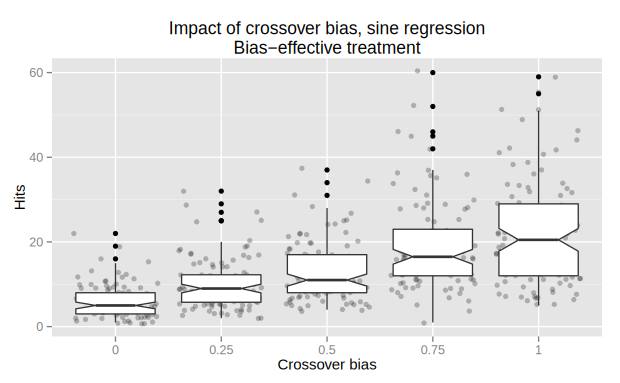
\includegraphics[width=0.45 \textwidth]{Plots/Sine_XO_impact_strong_boxplot.pdf}
\caption{Impact of crossover bias on the sine symbolic regression problem with binary tournaments, no elitism, and 
population size 10,240}
\label{fig:sineBiasResultsStrong}
\end{figure}

%> pairwise.wilcox.test(sine_strong_final$Hits, sine_strong_final$Bias)
%
%	Pairwise comparisons using Wilcoxon rank sum test 
%
%data:  sine_strong_final$Hits and sine_strong_final$Bias 
%
%     0       0.25    0.5     0.75  
%0.25 1.9e-07 -       -       -     
%0.5  4.0e-15 0.0017  -       -     
%0.75 < 2e-16 1.2e-12 8.9e-06 -     
%1    < 2e-16 1.3e-13 2.9e-07 0.1938
%
%P value adjustment method: holm 

%> pairwise.wilcox.test(sine_strong_final$Standardized.fitness, sine_strong_final$Bias)
%
%	Pairwise comparisons using Wilcoxon rank sum test 
%
%data:  sine_strong_final$Standardized.fitness and sine_strong_final$Bias 
%
%     0       0.25    0.5     0.75 
%0.25 3.6e-10 -       -       -    
%0.5  < 2e-16 2.7e-05 -       -    
%0.75 < 2e-16 5.0e-14 1.1e-05 -    
%1    < 2e-16 < 2e-16 2.9e-09 0.072
%
%P value adjustment method: holm 

Figure~\ref{fig:sineBiasResultsWeak} shows the results for the sine regression problem using tournament size 7, 0.1\% 
elitism, and smaller populations  of size 1,024. None of these differences are statistically significant using a 
pairwise Wilcoxon rank sum test.

\begin{figure}
\centering
\includegraphics[width=0.45 \textwidth]{Plots/Sine_XO_impact_weak_boxplot.pdf}
\caption{Impact of crossover bias on the sine symbolic regression problem with tournament size 7, 0.1\% elitism, and 
population size 1,024.}
\label{fig:sineBiasResultsWeak}
\end{figure}

Figures~\ref{fig:sineBiasFitnessVsGenStrong} and~\ref{fig:sineBiasFitnessVsGenWeak} show the change in fitness 
over time for the strong and weak configurations. In the strong configuration we get a really clean ``adding bias is 
good'' demonstration. In the weak configuration, the impact of crossover bias is quite minimal; \textbf{oddly, though, it 
does look like a crossover bias of 1.0 is worse by a little bit than everything else at the end, which is weird}. Figure~
\ref{fig:sineBiasFitnessVsGenT2E01P10K} shows fitness over time for the ``weak'' configuration with population size 
10,240 (instead of 1,024 for the ``normal'' weak configuration). Increasing the pop size definitely improves the 
performance by quite a lot (no surprise). The different bias levels are all essentially the same at the end of the 100 
generations, but there is definitely a spread around 15-20 generations that is a really clean ``more bias is better'' 
demonstration (\textbf{Do we care?}) except for the fact that 0.75 and 1.0 are essentially the same. \textbf{Do we 
want to include both Figures~\ref{fig:sineBiasFitnessVsGenWeak} and~\ref{fig:sineBiasFitnessVsGenT2E01P10K}? 
Do we want to combine them into a single graph (either just one graph, or as two ``panels'' like, e.g., in Figure~
\ref{fig:parentErrorsSine}?}

\begin{figure}
\centering
\includegraphics[width=0.45 \textwidth]{Plots/Sine_XO_fitness_vs_gen_strong.pdf}
\caption{Impact of crossover bias on the sine symbolic regression problem with binary tournaments, no elitism, and 
population size 10,240.}
\label{fig:sineBiasFitnessVsGenStrong}
\end{figure}

\begin{figure}
\centering
\includegraphics[width=0.45 \textwidth]{Plots/Sine_XO_fitness_vs_gen_weak.pdf}
\caption{Impact of crossover bias on the sine symbolic regression problem with tournament size 7, 0.1\% elitism, and 
population size 1,024.}
\label{fig:sineBiasFitnessVsGenWeak}
\end{figure}

\begin{figure}
\centering
\includegraphics[width=0.45 \textwidth]{Plots/Sine_XO_fitness_vs_gen_t2_e01_p10K.pdf}
\caption{Impact of crossover bias on the sine symbolic regression problem with tournament size 7, 0.1\% elitism, and 
population size 10,240.}
\label{fig:sineBiasFitnessVsGenT2E01P10K}
\end{figure}

\section{Discussion} \label{sec:Discussion}

Why does all this happen this way? For example, why does crossover bias have a much stronger effect when using 
binary tournaments than when using larger tournament sizes such as 7. One possible explanation is that with large 
tournaments, the difference in fitness between the two parents is likely to be closer, because the larger tournaments 
help ensure that both parents are from the more highly fit part of the population. To better understand this, blah, blah, 
blah \textbf{We need to turn this into actual text}.

\begin{figure}
\centering
\includegraphics[width=0.45 \textwidth]{Plots/Parent_errors_sine.pdf}
\caption{Plot of the errors of all individuals chosen as parents from some sine runs. \textbf{Explain this.} \textbf{Do we want/need this plot?}}
\label{fig:parentErrorsSine}
\end{figure}

Figure~\ref{fig:parentDiffsSine} shows the distribution of relative difference in parent errors in the sine regression 
problem. For each crossover event, the relative difference in parent errors is
\[
	|e_A - e_B] / (e_A + e_B)
\]
where $e_A$ and $e_B$ are the errors of the two chosen parents $A$ and $B$. This has a minimum value of 0 when 
the two errors are the same, and a maximum value approaching 1 for the case where one of the errors is nearly 0.

\begin{figure}
\centering
\includegraphics[width=0.45 \textwidth]{Plots/Parent_normalized_error_diffs_sine.pdf}
\caption{Plot of the normalized differences in parent errors from some sine runs. \textbf{Explain this}.}
\label{fig:parentDiffsSine}
\end{figure}

We see similar results for the K-Landscapes problem, as illustrated in Figures~\ref{fig:parentFitnessesKLandscapes} and~\ref{fig:parentDiffsKLandscapes}.

\begin{figure}
\centering
\includegraphics[width=0.45 \textwidth]{Plots/Parent_fitnesses_KLandscapes.pdf}
\caption{Plot of the fitnesses of all individuals chosen as parents from some K-Landscape runs. \textbf{Explain this.} \textbf{Do we want/need this plot?}}
\label{fig:parentFitnessesKLandscapes}
\end{figure}

\begin{figure}
\centering
\includegraphics[width=0.45 \textwidth]{Plots/Parent_normalized_fitness_diffs_KLandscapes.pdf}
\caption{Plot of the normalized differences in parent fitnesses from some K-Landscape runs. \textbf{Explain this}.}
\label{fig:parentDiffsKLandscapes}
\end{figure}

\section{Conclusions} \label{sec:Conclusions}

In most of these experiments we found better results with tournament sizes of 7 than with binary tournaments, and in 
general using larger tournaments appears to wash out much of the impact of crossover bias, so there's a fair question 
about whether one should just use larger tournaments and ignore crossover bias. \textbf{How do we respond to this? I 
think the answer is something like ``It doesn't hurt (at least in our experiments), and it sometimes helps, even for 
tournament size 7 and with elitism. For interesting problems, you also don't know in advance what your best parameter 
choices are, so it's at least worth including in your arsenal.''}

\section*{Acknowledgements}

\bibliographystyle{acm}
\bibliography{Research_2015}

\end{document}